\section{Algoritme til detektering af gang, løb og cykling}
\textit{kursiv indledning...}

\subsection{Design og implementering}
%Pseudo kode  (Flowcharts)
%Timers, interrupts, clocks, powermodes
%Clocks: tæller tid...
%interrupt: start/stop ny funktion
%Databehandling/filtrering
%Tjek om det er cykling - hvis ja, start gyro
%Delay → send data til GAP central hvert 15. minut


%%%%% Behandling af gyro data %%%%%
\begin{enumerate}
	\item Gyro sleep i 10 sek - vækkes af interrupt.
	\item Opsaml data i 2 sek.
	\item FFT af rå data.
	\item Find max y af (1)
	\item Find arrayplads (x) for (2) \textrightarrow omregn til Hz : (2)/(antal samples/fs)
	\item Integrer (1) fra (3)-1 til (3)+1.
	\item Integrer (1) over 20 samples.
	\item Udregn hvor stor en del af (5) som består af (4) \textrightarrow (4)/(5)*100 = anden i \%.
	\item Threshold: cykling = > 70\% \textrightarrow optag og gem i flash, < 70\% \textrightarrow optag accelerometer. 
\end{enumerate}




%%%%% Behandling af accelerometer data %%%%%
\begin{enumerate}
	\item Elliptisk filter af rå data.
	\item Divider (1) med 8 og kvadrer.
	\item Moving average på (2). 
	\item Plot (3) med thresholds: løb = >0,65 , gang = 0,65>0,04 , ingen aktivitet = >0,04 \textrightarrow optag og gem i flash.
\end{enumerate}




%%%%% Pseudo kode (Flowcharts) %%%%%



\begin{figure}[H]
	\centering
	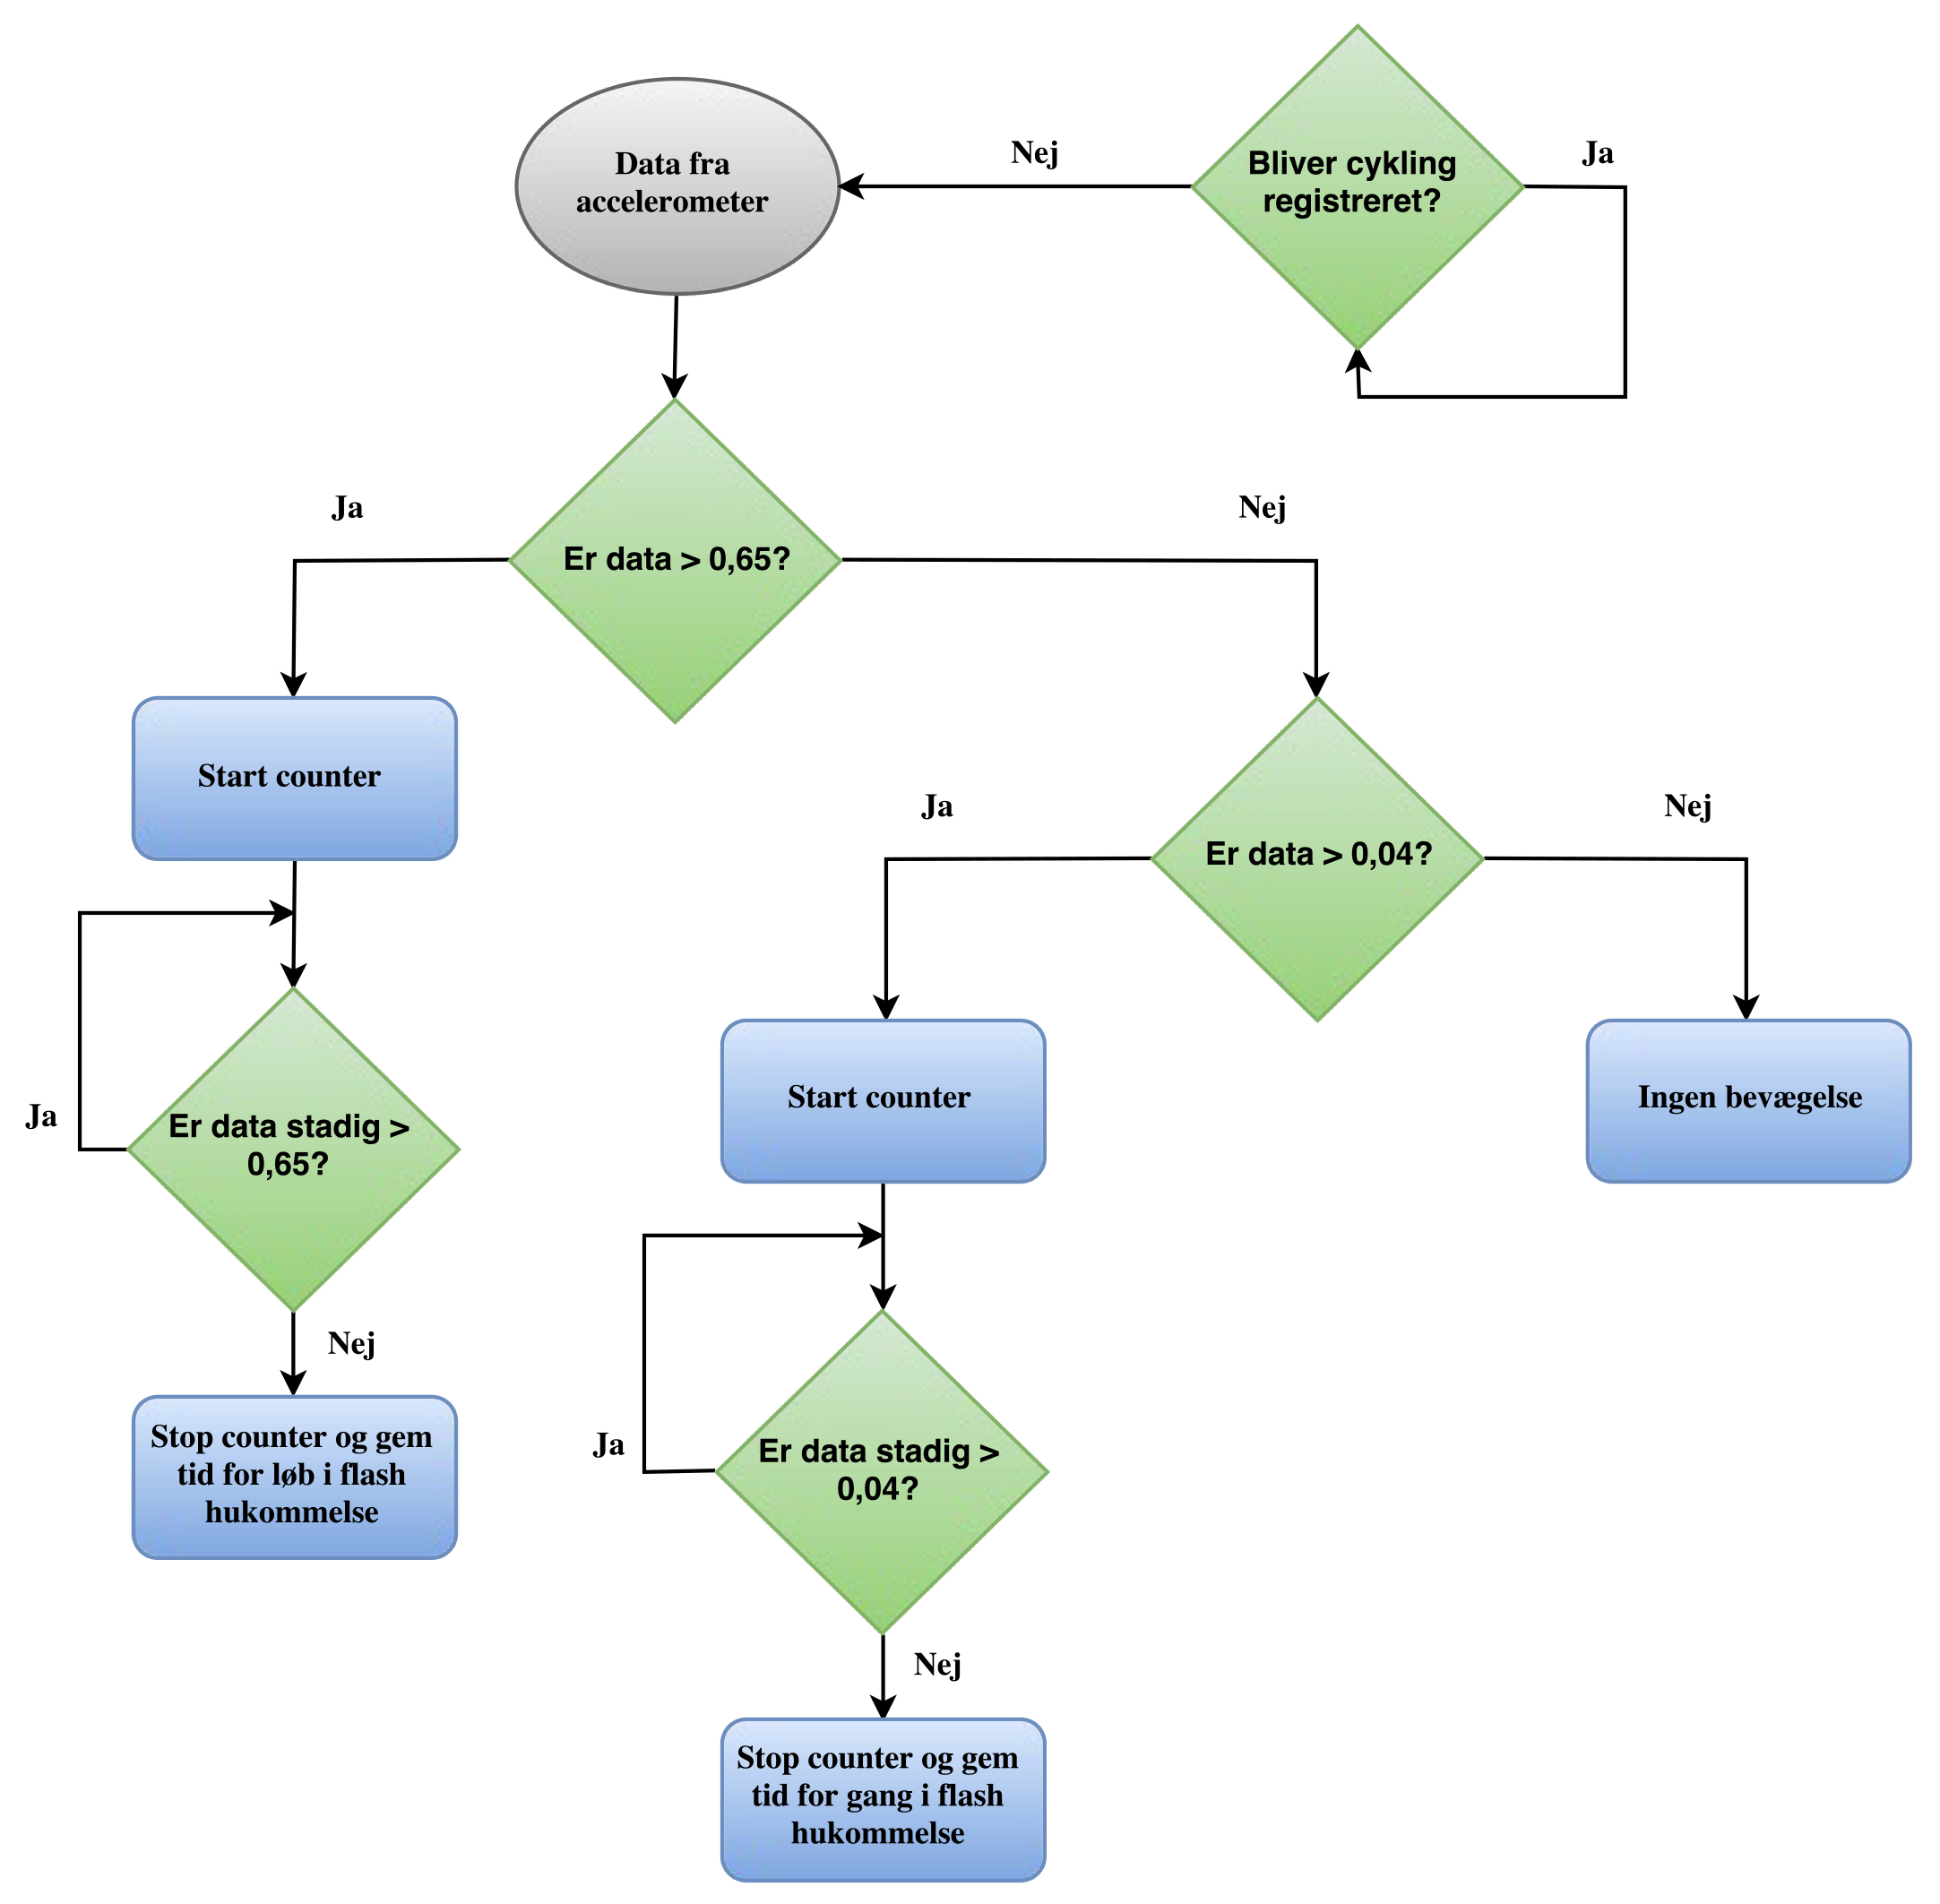
\includegraphics[scale=0.6]{figures/cDesign/algoritme.png}
	\caption{Flowchart over algoritmen}
	\label{fig:algoritme}
\end{figure}




\subsection{Test}


